% Original CSC302 teaching exposition based on Macbeth, Chapter 2, Sections 2.1--2.5.
% Source: https://hrmacbeth.github.io/math2001/02_Proofs_with_Structure.html
% Source snapshot: hrmacbeth/math2001 e660f42b13ddcb6d12b52ba036d6bd071a0cfb9b.
% New numerical variants are labelled with their source method's example number.
% CSC302 lecture slides adapted from Heather Macbeth, The Mechanics of Proof.
\documentclass[aspectratio=169,11pt]{beamer}
\usepackage[T1]{fontenc}
\usepackage{lmodern}
\usepackage{amsmath,amssymb,mathtools}
\usepackage{booktabs,array,listings,tikz}
\usetikzlibrary{arrows.meta,positioning,calc}
\definecolor{ProofNavy}{HTML}{18324F}
\definecolor{ProofTeal}{HTML}{007D82}
\definecolor{ProofPaper}{HTML}{F3F6F8}
\usetheme{default}
\setbeamercolor{normal text}{fg=ProofNavy,bg=white}
\setbeamercolor{structure}{fg=ProofTeal}
\setbeamercolor{frametitle}{fg=ProofNavy}
\setbeamercolor{block title}{fg=white,bg=ProofNavy}
\setbeamercolor{block body}{fg=ProofNavy,bg=ProofPaper}
\setbeamercolor{block title example}{fg=white,bg=ProofTeal}
\setbeamercolor{block body example}{fg=ProofNavy,bg=ProofPaper}
\setbeamerfont{frametitle}{size=\Large,series=\bfseries}
\setbeamertemplate{navigation symbols}{}
\setbeamertemplate{itemize item}{\small\textbullet}
\setbeamertemplate{footline}{%
  \leavevmode\hbox{%
  \begin{beamercolorbox}[wd=.86\paperwidth,ht=2.8ex,dp=1.2ex,leftskip=1.6em]{author in head/foot}%
    \scriptsize CSC302\quad\textbar\quad\insertshorttitle
  \end{beamercolorbox}%
  \begin{beamercolorbox}[wd=.14\paperwidth,ht=2.8ex,dp=1.2ex,rightskip=1.6em plus1fil]{date in head/foot}%
    \scriptsize\insertframenumber/\inserttotalframenumber
  \end{beamercolorbox}}}
\setbeamersize{text margin left=8mm,text margin right=8mm}
\lstdefinelanguage{Lean}{%
  morekeywords={example,theorem,lemma,def,by,calc,have,exact,apply,intro,intros,constructor,rcases,rfl,rw,ring,numbers,linarith,nlinarith,rel,extra,addarith,obtain,left,right,use,choose,dsimp,change,ext,fun,show,from,at,with,induction,case,decide,contradiction,push_neg,by_cases,by_contra,assumption,existsi,simp,simpa},
  sensitive=true,morecomment=[l]{--},morestring=[b]"}
\lstset{language=Lean,basicstyle=\ttfamily\small,keywordstyle=\color{ProofTeal}\bfseries,
  commentstyle=\color{gray},stringstyle=\color{ProofNavy},showstringspaces=false,
  columns=fullflexible,keepspaces=true,breaklines=true,frame=single,
  rulecolor=\color{ProofTeal!30},backgroundcolor=\color{ProofPaper},
  aboveskip=0.5em,belowskip=0.4em}
\newcommand{\N}{\mathbb{N}}
\newcommand{\Z}{\mathbb{Z}}
\newcommand{\Q}{\mathbb{Q}}
\newcommand{\R}{\mathbb{R}}
\newcommand{\coursechapter}[2]{%
  \title[Chapter #1: #2]{Chapter #1\\#2}%
  \subtitle{The Mechanics of Proof \textbar{} CSC302 lecture notes}%
  \author{Based on Heather Macbeth's textbook}%
  \date{}%
}
\newcommand{\sourcecredit}[1]{\par\vfill{\tiny Source: Heather Macbeth, \emph{The Mechanics of Proof}, #1.}}
\newcommand{\bookurl}{\url{https://hrmacbeth.github.io/math2001/}}
\hypersetup{colorlinks=true,urlcolor=ProofTeal,linkcolor=ProofNavy}

\coursechapter{2}{Proofs with structure}
\begin{document}

\begin{frame}\titlepage\end{frame}

\begin{frame}{What you will learn}
\begin{itemize}
\item Build and reuse an intermediate fact without losing track of the goal.
\item Apply an existing lemma by checking its hypotheses.
\item Use and prove statements involving $\lor$, $\land$, and $\exists$.
\item Organize cases and witnesses in both mathematical English and Lean.
\end{itemize}
\begin{block}{The recurring question}
What information does the hypothesis provide, and what information does the goal require?
\end{block}
\end{frame}

\section{2.1 Intermediate steps}
% Method: Examples 2.1.1--2.1.3.
\begin{frame}{2.1\quad A proof can have a dependency structure}
Suppose one hypothesis quickly determines $b$, while another relates $a$ to $b$.
\begin{center}
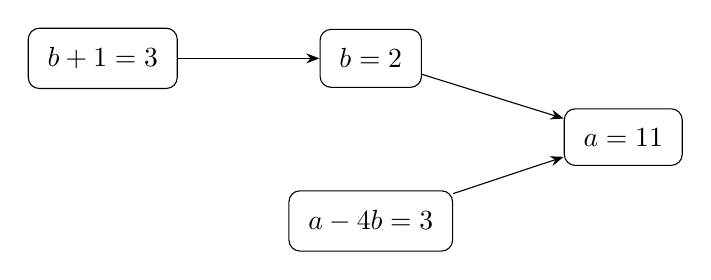
\begin{tikzpicture}[node distance=13mm and 18mm,
 every node/.style={draw,rounded corners,align=center,inner sep=7pt},
 >=Stealth]
\node (h2) {$b+1=3$};
\node[right=of h2] (hb) {$b=2$};
\node[below=of hb] (h1) {$a-4b=3$};
\node[right=of hb,yshift=-10mm] (goal) {$a=11$};
\draw[->] (h2)--(hb);
\draw[->] (hb)--(goal);
\draw[->] (h1)--(goal);
\end{tikzpicture}
\end{center}
Prove $b=2$ once, give it a name, and use it in the later calculation.
The diagram records which facts the conclusion depends on.
\sourcecredit{Section 2.1; method of Example 2.1.1}
\end{frame}

\begin{frame}{Worked example: an intermediate fact simplifies the calculation}
Let $a,b\in\R$, with $a-4b=3$ and $b+1=3$. Prove $a=11$.
\begin{block}{Intermediate fact}
Subtracting $1$ from $b+1=3$ gives $b=2$.
\end{block}
Now
\[
\begin{aligned}
a&=(a-4b)+4b&&\text{algebra}\\
 &=3+4\cdot2&&\text{the hypothesis and intermediate fact}\\
 &=11&&\text{arithmetic}.
\end{aligned}
\]
The word ``therefore'' should identify a real dependency: this calculation uses the value of $b$.
\sourcecredit{Section 2.1; numerical variant of Example 2.1.1}
\end{frame}

\begin{frame}[fragile]{Lean: \texttt{have} adds a proved fact to the context}
\begin{lstlisting}
example {a b : Real}
    (h1 : a - 4 * b = 3) (h2 : b + 1 = 3) : a = 11 := by
  have hb : b = 2 := by addarith [h2]
  calc
    a = (a - 4 * b) + 4 * b := by ring
    _ = 3 + 4 * 2 := by rw [h1, hb]
    _ = 11 := by numbers
\end{lstlisting}
\begin{itemize}
\item Before \texttt{have}: only \texttt{h1} and \texttt{h2} are available.
\item After it: \texttt{hb : b = 2} is also available.
\item The original goal is still $a=11$.
\end{itemize}
\sourcecredit{Example 2.1.1; numerical variant}
\end{frame}

% Cancellation: Examples 2.1.4 and 2.1.5.
\begin{frame}{Cancellation requires a reason}
\textbf{Example.} If $t\in\R$, $t^2=4t$, and $t\ge1$, then
\[
t\cdot t=4t,\qquad t\ne0,\qquad\text{hence }t=4.
\]
Without $t\ne0$, cancellation would discard the possible solution $t=0$.
\begin{block}{Cancelling squares is different}
If $u,v\ge0$ and $u^2\le v^2$, then $u\le v$.
Sign information matters: $(-3)^2=3^2$ does not imply $-3=3$.
\end{block}
The textbook tactic \texttt{cancel} checks the required side conditions.
On paper, state them when they are doing mathematical work.
\sourcecredit{Examples 2.1.4--2.1.5}
\end{frame}

\begin{frame}{Practice 2.1: identify an intermediate fact}
\begin{enumerate}
\item Let $m,n\in\Z$, with $m+2\le3n$ and $n\le4$. Prove $m\le10$.
\item Let $a,b\in\R$, with $a^2=b^2+9$ and $a\ge0$. Prove $a\ge3$.
\end{enumerate}
\vspace{1em}
Write down a useful intermediate inequality before writing the final sentence.
For the second problem, indicate where $a\ge0$ is needed.
\end{frame}

\begin{frame}{Practice 2.1: solution discussion}
\textbf{1.} First establish $m+2\le12$:
\[
m+2\le3n\le3\cdot4=12.
\]
Subtracting $2$ gives $m\le10$.
\medskip

\textbf{2.} First establish the comparison of squares:
\[
a^2=b^2+9\ge9=3^2.
\]
Since $a$ and $3$ are nonnegative, this implies $a\ge3$.
Without $a\ge0$, the instance $a=-3,b=0$ would contradict the conclusion.
\end{frame}

\section{2.2 Invoking lemmas}
\begin{frame}{2.2\quad A lemma converts one task into another}
A lemma is a previously proved implication that may be reused.
\begin{center}
\begin{tabular}{lll}
\toprule
Lemma & What it needs & What it gives \\
\midrule
\texttt{ne\_of\_lt} & $a<b$ & $a\ne b$ \\
\texttt{ne\_of\_gt} & $a>b$ & $a\ne b$ \\
\texttt{le\_antisymm} & $a\le b$ and $b\le a$ & $a=b$ \\
\bottomrule
\end{tabular}
\end{center}
\begin{itemize}
\item \texttt{apply L} works backward: replace the goal by the hypotheses needed by $L$.
\item \texttt{have h := L ...} works forward: store the conclusion obtained from supplied inputs.
\item \texttt{exact h} closes a goal already proved by $h$.
\end{itemize}
\sourcecredit{Section 2.2}
\end{frame}

\begin{frame}[fragile]{Worked example: prove a stronger comparison}
Let $x\in\Q$ and suppose $5x=3$. To prove $x\ne1$, it suffices to prove $x<1$:
\[
x=\frac{5x}{5}=\frac35<1.
\]
\begin{lstlisting}
example {x : Rat} (h : 5 * x = 3) : Not (x = 1) := by
  apply ne_of_lt
  calc
    x = 5 * x / 5 := by ring
    _ = 3 / 5 := by rw [h]
    _ < 1 := by numbers
\end{lstlisting}
The new goal after \texttt{apply ne\_of\_lt} is $x<1$.
\sourcecredit{Section 2.2; numerical variant of Example 2.2.1}
\end{frame}

% Theorem and argument: Example 2.2.3.
\begin{frame}{Worked example: squeeze a square to zero}
Let $a,b\in\R$ and suppose $a^2+b^2=0$. Prove $a^2=0$.
\begin{enumerate}
\item A square is nonnegative, so $0\le a^2$.
\item The other square is nonnegative, so
\[
a^2\le a^2+b^2=0.
\]
\item Combining $a^2\le0$ and $0\le a^2$ gives $a^2=0$.
\end{enumerate}
\begin{block}{Lean structure}
\texttt{apply le\_antisymm} creates two goals.
Both must be proved; the first is an upper bound and the second a lower bound.
\end{block}
\sourcecredit{Example 2.2.3}
\end{frame}

\begin{frame}{Practice 2.2: choose the lemma}
\begin{enumerate}
\item Let $q\in\Q$, with $4q\le8$ and $2q\ge4$. Prove $q=2$.
\item Let $m\in\Z$, with $m+3=7$. Prove $3m\ne9$.
\end{enumerate}
\vspace{1em}
Which lemma should be applied first? What new goal or goals will it create?
\end{frame}

\begin{frame}{Practice 2.2: solution discussion}
\textbf{1.} Use antisymmetry. Its two required inequalities are
\[
q=\frac{4q}{4}\le\frac84=2,
\qquad
q=\frac{2q}{2}\ge\frac42=2.
\]
Hence $q=2$.
\medskip

\textbf{2.} Since $m+3=7$, we have $m=4$. Therefore
\[
3m=3\cdot4=12>9.
\]
Use \texttt{ne\_of\_gt} to obtain $3m\ne9$.
\end{frame}

\section{2.3 Or and proof by cases}
\begin{frame}{2.3\quad ``Or'' has different roles in a hypothesis and a goal}
$P\lor Q$ means that at least one of $P,Q$ is true; both may be true.
\begin{columns}[T]
\begin{column}{.48\textwidth}
\begin{block}{Using $P\lor Q$}
Prove the target assuming $P$.
Then prove it assuming $Q$.
Both cases are required because you do not know which holds.
\end{block}
\end{column}
\begin{column}{.48\textwidth}
\begin{block}{Proving $P\lor Q$}
It is enough to prove one alternative.
Choose \texttt{left} for $P$ or \texttt{right} for $Q$.
The chosen alternative may depend on the current case.
\end{block}
\end{column}
\end{columns}
\medskip
Facts introduced inside one case are available only in that case.
\sourcecredit{Examples 2.3.1--2.3.4}
\end{frame}

\begin{frame}{Worked example: the same goal in two cases}
Let $x,y\in\R$, and suppose $x=2$ or $y=-2$.
Prove $xy+2x=2y+4$.
\begin{block}{Case 1: $x=2$}
\[
xy+2x=2y+2\cdot2=2y+4.
\]
\end{block}
\begin{block}{Case 2: $y=-2$}
\[
xy+2x=x(-2)+2x=0=2(-2)+4=2y+4.
\]
\end{block}
Each branch reaches the entire original goal.
\sourcecredit{Section 2.3; method of Example 2.3.1}
\end{frame}

\begin{frame}{Worked example: create a useful disjunction}
Let $x\in\R$ and suppose $x^2-5x+6=0$. Prove $x=2$ or $x=3$.
\begin{enumerate}
\item Factor the known polynomial:
\[
(x-2)(x-3)=x^2-5x+6=0.
\]
\item Use the zero-product property: $uv=0$ implies $u=0$ or $v=0$.
\item If $x-2=0$, then $x=2$, establishing the left alternative.
\item If $x-3=0$, then $x=3$, establishing the right alternative.
\end{enumerate}
The new disjunction is an intermediate fact; it is not an extra assumption.
\sourcecredit{Section 2.3; numerical variant of Example 2.3.4}
\end{frame}

\begin{frame}[fragile]{Lean: make the case structure visible}
\begin{lstlisting}
example {x : Real} (h : x ^ 2 - 5 * x + 6 = 0) :
    Or (x = 2) (x = 3) := by
  have hf : (x - 2) * (x - 3) = 0 := by
    calc
      (x - 2) * (x - 3) = x ^ 2 - 5 * x + 6 := by ring
      _ = 0 := h
  have hz := eq_zero_or_eq_zero_of_mul_eq_zero hf
  cases hz with
  | inl h2 =>
      left
      addarith [h2]
  | inr h3 =>
      right
      addarith [h3]
\end{lstlisting}
\sourcecredit{Section 2.3; ASCII syntax for the case structure}
\end{frame}

% Mathematical fact and method: Example 2.3.2; nested integer cases: 2.3.5.
\begin{frame}{A discrete gap gives an exhaustive case split}
\textbf{Claim.} No natural number has square $2$.

For $n\in\N$, either $n\le1$ or $2\le n$.
\begin{itemize}
\item If $n\le1$, then $n^2\le1<2$.
\item If $2\le n$, then $n^2\ge4>2$.
\end{itemize}
Thus in either case $n^2\ne2$.
\begin{block}{What changes for integers?}
Handle negative $n$ by considering the nonnegative number $-n$ and using $(-n)^2=n^2$.
\end{block}
The split is exhaustive because no natural number lies strictly between $1$ and $2$.
\sourcecredit{Examples 2.3.2 and 2.3.5}
\end{frame}

\begin{frame}{Practice 2.3: create the right cases}
\begin{enumerate}
\item If $x\in\R$ and $x^2-2x-3=0$, prove $x=-1$ or $x=3$.
\item For every $n\in\N$, prove $n^2\ne6$.
\end{enumerate}
\vspace{1em}
Explain why your cases cover all possibilities.
For the first problem, say which alternative of the goal each case proves.
\end{frame}

\begin{frame}{Practice 2.3: solution discussion}
\textbf{1.} Since
\[
(x+1)(x-3)=x^2-2x-3=0,
\]
we have $x+1=0$ or $x-3=0$.
These give $x=-1$ and $x=3$, respectively.
\medskip

\textbf{2.} Split into $n\le2$ and $3\le n$.
\[
n\le2\implies n^2\le4<6,
\qquad
3\le n\implies n^2\ge9>6.
\]
Every natural number lies in one of these cases.
\end{frame}

\section{2.4 And}
\begin{frame}{2.4\quad An ``and'' packages two facts}
$P\land Q$ means that both $P$ and $Q$ hold.
\begin{columns}[T]
\begin{column}{.48\textwidth}
\begin{block}{Using $P\land Q$}
Extract both facts and use them in the same proof.
For a Lean hypothesis \texttt{h}, its components are \texttt{h.1} and \texttt{h.2}.
\end{block}
\end{column}
\begin{column}{.48\textwidth}
\begin{block}{Proving $P\land Q$}
Prove both components.
\texttt{constructor} creates two goals, or \texttt{And.intro} combines two existing proofs.
\end{block}
\end{column}
\end{columns}
\medskip
An inequality chain such as $0<x<1$ abbreviates $0<x\land x<1$.
\sourcecredit{Section 2.4}
\end{frame}

\begin{frame}{Worked example: solve for both variables}
Let $x,y\in\Q$, with $x+y=8$ and $x+2y=11$.
Prove $x=5$ and $y=3$.
\begin{enumerate}
\item First find a reusable intermediate fact:
\[
y=(x+2y)-(x+y)=11-8=3.
\]
\item Use it to obtain the other component:
\[
x=(x+y)-y=8-3=5.
\]
\item We have now proved both parts of the conjunction.
\end{enumerate}
Establishing $y=3$ before splitting the goal lets both parts refer to it.
\sourcecredit{Section 2.4; methods of Examples 2.4.1 and 2.4.3}
\end{frame}

\begin{frame}[fragile]{Lean: extract, derive, and repackage}
\begin{lstlisting}
example {x y : Rat}
    (h : And (x + y = 8) (x + 2 * y = 11)) :
    And (x = 5) (y = 3) := by
  have hy : y = 3 := by
    calc
      y = (x + 2 * y) - (x + y) := by ring
      _ = 11 - 8 := by rw [h.2, h.1]
      _ = 3 := by numbers
  have hx : x = 5 := by
    calc
      x = (x + y) - y := by ring
      _ = 8 - 3 := by rw [h.1, hy]
      _ = 5 := by numbers
  exact And.intro hx hy
\end{lstlisting}
\sourcecredit{Section 2.4; new numerical example}
\end{frame}

\begin{frame}{Practice 2.4: unpack and repack}
\begin{enumerate}
\item Let $r,s\in\R$. Assume the single conjunction
\[
r+s\le3\ \land\ r-s\le5.
\]
Prove $r\le4$.
\item Let $p\in\Z$, with $p-1\ge3$. Prove $p\ge4\land p^2\ge16$.
\end{enumerate}
Which proof uses a conjunction? Which constructs a conjunction?
\end{frame}

\begin{frame}{Practice 2.4: solution discussion}
\textbf{1.} Both components of the hypothesis are available:
\[
r=\frac{(r+s)+(r-s)}2\le\frac{3+5}2=4.
\]
\textbf{2.} The hypothesis gives $p\ge4$ by adding $1$.
In particular $p\ge0$, so squaring preserves the comparison:
\[
p^2\ge4^2=16.
\]
These prove the two components of $p\ge4\land p^2\ge16$.
\end{frame}

\section{2.5 Existence proofs}
\begin{frame}{2.5\quad An existential statement promises a witness}
\[
\exists x\in D,\ P(x)
\]
asserts that at least one object $x$ in the domain $D$ satisfies $P$.
\begin{columns}[T]
\begin{column}{.48\textwidth}
\begin{block}{Using an existential}
Introduce a witness $x$ and its promised property $P(x)$.
You may use that property, but may not assume anything else about the witness.
\end{block}
\end{column}
\begin{column}{.48\textwidth}
\begin{block}{Proving an existential}
Choose a particular witness $w\in D$ and prove $P(w)$.
Lean's \texttt{use w} leaves the property as the new goal.
\end{block}
\end{column}
\end{columns}
\sourcecredit{Section 2.5}
\end{frame}

\begin{frame}{Worked example: use a witness supplied by the hypothesis}
Let $a\in\Q$. Suppose there is a rational number $b$ with $a=b^2+2$.
Prove $a>0$.
\begin{enumerate}
\item Introduce such a number $b$, with its property $a=b^2+2$.
\item Every rational square is nonnegative, so
\[
a=b^2+2\ge2>0.
\]
\end{enumerate}
\begin{block}{The witness is not yours to choose}
The hypothesis does not say that $b=0$.
It gives some $b$ that satisfies the property, and the proof must work for that witness.
\end{block}
\sourcecredit{Section 2.5; numerical variant of Example 2.5.1}
\end{frame}

% Witness construction: Examples 2.5.4, 2.5.6, and 2.5.7.
\begin{frame}{Worked example: construct a point between two numbers}
Let $p,q\in\R$ and suppose $p<q$. Prove that there exists $x$ with $p<x<q$.
\begin{block}{Choice of witness}
Take $x=(p+q)/2$.
\end{block}
Check both required inequalities:
\[
p=\frac{p+p}{2}<\frac{p+q}{2},
\qquad
\frac{p+q}{2}<\frac{q+q}{2}=q.
\]
Both steps use $p<q$ and division by the positive number $2$.
The domain matters: there is no integer strictly between $2$ and $3$.
\sourcecredit{Example 2.5.7}
\end{frame}

\begin{frame}[fragile]{Lean: a witness becomes a concrete verification task}
\begin{lstlisting}
example : Exists (fun n : Int => 9 * n = 54) := by
  use 6
  numbers

example (x : Real) : Exists (fun y : Real => y > x) := by
  use x + 1
  extra
\end{lstlisting}
In the first proof, \texttt{use 6} replaces an existence goal by $9\cdot6=54$.

In the second proof, the witness is a formula depending on the given $x$.
\sourcecredit{Section 2.5; methods of Examples 2.5.3--2.5.4}
\end{frame}

\begin{frame}{Practice 2.5: propose and verify witnesses}
\begin{enumerate}
\item Find integers $m,n$ with $m^2+n^2=65$.
\item Given any integer $a$, prove that some integers $m,n$ satisfy
\[
m^2-n^2=2a+1.
\]
\item Given a real number $t$, prove that some real $u$ satisfies $u<t$.
\end{enumerate}
Write down the proposed witness before checking the property.
\end{frame}

\begin{frame}{Practice 2.5: solution discussion}
\textbf{1.} Take $m=4$ and $n=7$:
\[
4^2+7^2=16+49=65.
\]
\textbf{2.} Take $m=a+1$ and $n=a$:
\[
(a+1)^2-a^2=a^2+2a+1-a^2=2a+1.
\]
\textbf{3.} Take $u=t-1$. Since $-1<0$, we have $t-1<t$.
\medskip

Each proof contains two ingredients: an object of the required type and a verification of its property.
\sourcecredit{Problem 2 follows Example 2.5.6}
\end{frame}

\begin{frame}{Chapter 2: match the logical form to the proof action}
\begin{center}
\begin{tabular}{lll}
\toprule
Form & Use as a hypothesis & Prove as a goal \\
\midrule
$P\lor Q$ & Handle both cases & Establish one alternative \\
$P\land Q$ & Extract both facts & Establish both components \\
$\exists x,\ P(x)$ & Introduce witness and property & Choose and verify a witness \\
\bottomrule
\end{tabular}
\end{center}
\begin{itemize}
\item \texttt{have} records intermediate work.
\item A lemma application must discharge all of its required hypotheses.
\item Case assumptions and witness properties have a scope; respect it.
\end{itemize}
\end{frame}

\begin{frame}{Reading and source references}
Heather Macbeth, \emph{The Mechanics of Proof}, Chapter 2:
\begin{itemize}
\item 2.1 Intermediate steps
\item 2.2 Invoking lemmas
\item 2.3 ``Or'' and proof by cases
\item 2.4 ``And''
\item 2.5 Existence proofs
\end{itemize}
\small
\url{https://hrmacbeth.github.io/math2001/02_Proofs_with_Structure.html}
\par\medskip
Companion code: \url{https://github.com/hrmacbeth/math2001}
\par\medskip
These slides independently organize the chapter's proof methods and include new numerical practice.
\end{frame}
\end{document}
